\documentclass[12pt,preprint]{aastex}
\usepackage{graphicx}


%%%%%%%%%%%%%%%%%%%%%%%%%%%%%%%%%%%%%%%%%%%%%%%%%%%%
%%% author-defined commands
\newcommand\x         {\hbox{$\times$}}
\newcommand\othername {\hbox{$\dots$}}
\def\eq#1{\begin{equation} #1 \end{equation}}
\def\eqarray#1{\begin{eqnarray} #1 \end{eqnarray}}
\def\eqarraylet#1{\begin{mathletters}\begin{eqnarray} #1 %
                  \end{eqnarray}\end{mathletters}}
\def\mic              {\hbox{$\mu{\rm m}$}}
\def\about            {\hbox{$\sim$}}
\def\Mo               {\hbox{$M_{\odot}$}}
\def\Lo               {\hbox{$L_{\odot}$}}
\def\comm#1           {{\tt (COMMENT: #1)}}
%%%%%%%%%%%%%%%%%%%%%%%%%%%%%%%%%%%%%%%%%%%%%%%%%%%%


\begin{document}

\title{Level 2 Photometric Calibration for the LSST Survey}

\author{
Lynne Jones, David Burke, \v{Z}eljko Ivezi\'{c}, and the Photometric Calibration Team
}

%\begin{abstract}
%\end{abstract}


\section{Introduction}


Two levels of LSST photometric calibration will be carried out at
differing cadences and with differing performance targets. A nightly
data calibration based on the best available set of prior calibrated
observations will provide “best-effort” precision and accuracy. This
calibration will be used for quality assurance, generation of alerts
to transients, and other quantities appropriate for Level 1 Data
Products.  A more complete analysis will recalibrate the data
accumulated by the survey at periodic “Data Release” dates (Level 2 in
LSST data management terminology.)  It is this repeated calibration of
the accumulated survey that will be held to the survey requirements
for photometric repeatability, uniformity, and accuracy.  This
document describes the calibration requirements and processes for the
Level 2 photometric calibration.

\section{Photometric Requirements}

The LSST Science Requirements Document (SRD) specifies that the survey
must deliver photometry with the following characteristics:
\begin{enumerate}
\item{Repeatability of 5 millimags in $gri$, 7.5 millimags in $uzy$,
for bright unresolved sources.  This specifies the distribution of
random photometric errors ($\sigma$) and constrains both the
repeatability of extracting counts from images and the ability to
monitor (or model) the changes in normalized system response
($\phi$). It could be thought of as making the photometry of a single
source consistent over time. \label{repeatability_req}}
\item{Uniformity of 10 millimags in $grizy$, and up to 20 millimags in
$u$, again for bright unresolved sources. This places a constraint on
the stability of the photometric system across the sky and places an
upper limit on various systematic errors, such as a correlation of
internal photometric zero-point error with the position on a
sensor. This makes the photometry of many sources comparable over the
entire sky, which when combined with the previous requirements creates
a stable photometric system across the sky and over time, in a single
filter. \label{uniformity_req}}
\item{Band-to-band zero-point calibration for main sequence stars of 5
millimags for any color not involving $u$ band, 10 millimags for
colors constructed with $u$ band photometry. This constrains the upper
limit of the systematic error in the measurement of the system
throughput as a function of wavelength. This requirement ties
photometric measurements in different filters together, enabling
colors to be measured for sources with unknown SEDs or (for sources
with known SEDs) magnitudes in different filters to be directly
compared. \label{color_req}}
\item{Zero-point calibration with respect to an external system of 10
millimags. This requirement ties LSST internal photometry to a
physical scale, and places a constraint on the upper limit of the
systematic error in the measurement of the total system
throughput. This final step enables LSST photometry to be compared
with photometry from other telescopes using other photometric
systems. \label{abs_req}}
\end{enumerate}

Requirements \ref{repeatability_req} and \ref{uniformity_req} must be
met by compensating for changes in system sensitivity as a function of
time, location in the sky or focal plane, and result in a relative
calibration within a single filter. Requirements \ref{color_req}
and \ref{abs_req} require additional measurements of sources with
known colors and absolute magnitudes, where these additional
measurements result in a relative calibration from filter to filter as
well as an absolute physical scale for the overall system.

Only photometric measurements released as part of the data release
products (generated annually) will be held to the requirements
above. On a nightly timescale, photometric measurements needed for
alert generation, quality assurance, or other short-timescale data
products will be generated to ``best-effort'' precision and accuracy
using the best-available prior calibrated observations.

\section{Overview of the photometric calibration process}

The photometric requirements described above are a factor of 2 better
than those achieved by previous wide-field surveys operating on
primarily photometric nights. To reach this level of precision using
observations taken under a wide variety of conditions (including
non-photometric nights) requires a new approach. This is possible by
gathering additional data on the wavelength dependence of the
throughput of the hardware system and the atmosphere and by leveraging
the multiple observations of many stars that LSST will
gather. Traditional photometric calibration uses a set of standard
stars, observed at a range of airmasses in between science
observations, to calculate zeropoint offsets and perhaps a single
color-dependent extinction term for the science images. Calibration of
LSST magnitudes to SRD levels, under conditions with up to XXX cloud
extinction, would require standard stars in every CCD of every
exposure: this standard star network is thus necesssarily defined as the
non-variable, isolated, bright stars observed within LSST itself. In
addition, when considering the possibility of $>1\%$ variations in the
filter bandpasses across the field of view and/or the strong effects
of water band absorption in the $y$ band (see
Fig~\ref{fig:colorexamples} CREATE FIGURE), it becomes clear that LSST
must measure and correct for wavelength-dependent effects to a much
higher level than previous surveys. This section describes and motivates our
photometric calibration approach. 

The end goal of photometric calibration is to be able to translate
`counts measured in a particular image' into `photons above the
atmosphere', removing the signatures introduced by the atmosphere, the
telescope, the detector, and (potentially) data processing. So, let us
first consider how the light from a source is translated into
counts. 

Given $F_\nu(\lambda)$, the specific flux of an object {\it at
the top} of the atmosphere, at a position described by ($alt$,$az$),
the flux transmitted through the atmosphere to the telescope pupil is
\begin{equation}
\label{eqn:Fpupil}
                      F_\nu^{pupil}(\lambda,alt,az,t) = F_\nu(\lambda) \, S^{atm}(\lambda,alt,az,t),
\end{equation}
where $S^{atm}(\lambda,alt,az)$ is the (dimensionless) probability that a photon of 
wavelength $\lambda$ makes it through the atmosphere,
\begin{equation}
\label{eqn:atmTau}
                        S^{atm}(\lambda,alt,az,t)   = {\rm e}^{-\tau^{atm}(\lambda,alt,az,t)}.
\end{equation}
Here $\tau^{atm}(\lambda,alt,az)$ is the optical depth of the
atmospheric layer at wavelength $\lambda$ towards the position
($alt$,$az$).  Observational data show that $\tau^{atm}$'s dependency
on wavelength is slowly varying with time ($t$) (on the order of
5-10\% over an hour near the water bands) and position ($alt$,$az$)
(primarily a function of airmass, but additional variation on the
scale of tens of degrees can be detected due to water vapor
absorption) (LSST-5367?), under `typical' observing conditions.  
Clouds represent an additive gray (non-wavelength dependent)
contribution to $\tau^{atm}$ which can introduce a strong variation of
$\tau^{atm}$ on much smaller angular scales and short timescales (on
the order of 2-10\% of the total extinction at $1^{\circ}$ scales,
variable within minutes) (Ivezic2007). Under ``photometric''
atmospheric conditions, most of $\tau^{atm}$ variation is a smooth
function of $alt$, or airmass, however LSST will need to observe under
a wide variety of non-photometric conditions in order to achieve its
survey goals.

Note that while both $F_\nu(\lambda,t)$ and $\tau^{atm}(\lambda,alt,az,t)$ 
could vary more quickly than the standard LSST exposure time of 15
seconds, it is assumed here that all quantities are averaged over some
short exposure time and that $t$ indicates that the quantities could
vary from exposure to exposure. 

Given $F_\nu^{pupil}(\lambda,alt,az,t)$, the counts recorded at a
position within the field of view described by ($x$,$y$) can be
written as
\begin{equation}
\label{eqn:Fpupil2counts}
    C_b(alt,az,x,y,t) = C \, \int_0^\infty {F_\nu^{pupil}(\lambda,alt,az,t) \, S_b^{sys}(\lambda,x,y,t) \lambda^{-1}d\lambda}.
\end{equation}
Here, $S_b^{sys}(\lambda,x,y,t)$ is the (dimensionless) probability
that a photon will be converted into an ADU count, and the term
$\lambda^{-1}$ comes from the conversion of energy per unit frequency
into the number of photons per unit wavelength ($b=ugrizy$). The
dimensional conversion constant $C$ is
\begin{equation}
\label{eqn:Cconstant}
        C = {\pi D^2 \Delta t \over 4 g h }  
\end{equation}
where $D$ is the effective primary mirror diameter, $\Delta t$ is the
exposure time, $g$ is the gain of the readout electronics (number of
photoelectrons per ADU count, a number greater than one), and $h$ is
the Planck constant. The system response function,
$S_b^{sys}(\lambda,x,y)$, includes the (multiplicative) effects of the
mirror reflectance, transmission. In general, the wavelength-dependent
variations in $S_b^{sys}$ change slowly and over spatial scales much
larger than the PSF; over periods of months, the mirror reflectance
and filter transmission will degrade as their coatings
age. $S_b^{atm}$ is likely to also show a wavelength-dependent spatial
variation ($x$, $y$), due to irregularities in the filter material and
variations in the incident angle of incoming light, which would vary
on a similar time and spatial scale (Regnault ref). Spatial variations
in $S_b^{sys}$ that are independent of wavelength can occur more
rapidly, on the timescale of a day, and on a pixel level spatial
scale. Dust on the dewar window or filter or detector sensitivity
variations on the pixel-to-pixel scale can be treated as
wavelength-independent. 
%A more rapid wavelength-dependent variation in
%detector sensitivity (especially at the very red wavelengths in the
%$y$ band) results from variations in the temperature of the detector,
%but with little or no spatial variation.

From equation~\ref{eqn:Fpupil2counts} and the paragraphs above, we can see
that the generation of counts $C_b(alt,az,x,y,t)$ from photons is
imprinted with many different kinds of effects, which have different
scales of variability over time ($t$), spatial scale ($alt$, $az$ or
$x$, $y$), and wavelength ($\lambda$), suggesting that it is possible
and even beneficial to separate these effects for calibration
purposes. Wavelength-dependent effects can be considered variations in
the {\it shape} of the bandpass; gray-scale effects can be considered
variations in the {\it normalization} of the bandpass. Furthermore,
variations in the bandpass caused by the hardware system can be
separated from variations in the bandpass caused by atmospheric
throughput, and measured with different methods. 

First, consider the variations in $S_b^{sys}(\lambda,x,y,t)$, which
vary on timescales of a day or more.  We can further divide and
correct the measured counts for variations in
$S_b^{sys}(\lambda,x,y,t)$, the throughput in the hardware system, as
follows. Using a dome-screen system that is capable of producing light
at a range of individual wavelengths (the ``stubbsometer''), we can
measure the sensitivity of the mirror/lens/filter/detector system as a
function of $x$,$y$ at each wavelength, producing a series of `narrow
band flat fields'. While it would be possible to use these as a
standard flat field (after choosing a particular method to combine the
measurements at different wavelengths), it is not possible to generate
all the necessary narrow band flats each night; scanning through all 6
filters at 1nm intervals requires tens of hours. However, since the
wavelength-dependent effects are expected to vary slowly over time, we
can instead plan to only produce narrow band flat fields every 30
days. Using standard white-light flat fields for each filter acquired
at the start and end of observing on each night, we can also correct
for the much more rapidly changing wavelength-independent effects
(dust accumulation, pixel-to-pixel sensitivity variations, etc.) that
occur primarily on scales smaller than the PSF. The images are
corrected for gray-scale effects with the white-light flat field, and
also corrected for the wavelength-dependent effects in system
throughput measured from the narrow band flats.

Next, considering $S_b^{atm}(\lambda,alt,az,t)$, we can again
separate the wavelength-dependent variations, which occur over
spatial scales larger than the field of view and several minute timescales, from the gray
variations due to clouds, which occur over much smaller spatial and
time scales. By using an auxiliary telescope equipped with a
spectroscope to examine bright stars with known spectral energy
distributions (primarily white dwarfs due to their lack of spectral
lines, stars that would be near but not necessarily in the field of
view of the main telescope), we can measure the absorption lines in
the atmosphere every 5--10 minutes. These observations are used as
constraints for MODTRAN atmospheric models, generating simpler
representations of the atmospheric throughput which can be
interpolated to provide models of the wavelength-dependence of
$S_b^{atm}(\lambda,alt,az,t)$ in each observation. In order to correct
for the higher frequency gray-scale variations in $S_b^{atm}$, we must
use the observations of the stars themselves; because we have many repeat
observations of many stars, we can use a `self-calibration' procedure
similar to the ubercal method used with SDSS Stripe 82 data
(Padmanabhan REF). By selecting non-variable, main-sequence stars
from each observation, then minimizing the least-squares differences
between these observations, we can determine the extinction due to
clouds within each chip, then apply this extinction to all other
photometric measurements from the same observation. 

To summarize the LSST photometric calibration: pixel-to-pixel gray sensitivity variations are corrected
using white-light flat fields, wavelength-dependent
variations of the hardware system across the field of view are
corrected with narrow band flats generated by the ``stubbsometer''
dome screen, wavelength-dependent variations due to the atmosphere are
corrected with MODTRAN models generated using the auxiliary telescope,
and gray variations on the scale of a CCD due to clouds are corrected
using self-calibration. Each of these steps are necessary to achieve
0.5\% precision in repeat photometry and 1\% precision in photometric
stability across the sky (requirements \ref{repeatability_req} and
\ref{uniformity_req} ). It is worth noting that the procedure
described above generates `natural magnitudes' which could be thought
of as 
\begin{eqnarray}
\label{eqn:natmags}
m^{nat} & = &-2.5 \, log_{10} \, (C_{b, raw}(alt,az,x,y,t))  \\ 
 & & + \delta z_{ff}(x,y,t) + \delta k_{stubbsometer}(\lambda,x,y,t)  \nonumber \\  
 & &+ \delta z_{selfcalib}(alt,az,t)  + \delta
 k_{MODTRAN}(\lambda,alt,az,t)  \nonumber
\end{eqnarray}
where the counts from the object in the image are translated to an internally consistent magnitude
through corrections from the flat field, stubbsometer, atmospheric models and
self-calibration procedures. The wavelength-dependent corrections,
$\delta k$, are equivalent to correcting the {\it shape} of the
bandpass in each filter to a `standard' bandpass (which will be
defined during commisioning), while the wavelength independent
corrections, $\delta z$, are equivalent to correcting the {\it
normalization} of the bandpass to a common standard.  These `natural
magnitudes' are not, however, tied to an external physical scale, nor
are measurements in one filter tied to measurements in another filter
(requirements \ref{color_req} and \ref{abs_req}).  

To fulfill these last two requirements a further set of measurements
are needed. In all filters, a set of objects with a well-known
spectral type (such as main sequence stars or white dwarfs, preferably
with direct observations of the SED of the specific object) must be
observed and calibrated, in individual filters, as above. The prior
knowledge of each SED is combined with the `standard bandpass' shape
to generate synthetic color photometry. These synthetic colors are
then compared with the calibrated natural magnitudes from
Eqn~\ref{eqn:natmags} to calculate $\Delta_{b-r}$, the corrections
needed to tie measurements in each filter together (referenced to $r$
band).  At this point, only one final measurement is necessary to tie
the entire system to an external physical scale: an $r$ band LSST
natural magnitude measurement of an absolutely calibrated source on a
photometric night. Although in theory these last two steps could be
done with a single externally calibrated object, on a single
photometric night, a larger set of external reference objects spread
throughout the sky will be used to reduce systematic errors. This then
produces a final magnitude, 
\begin{equation}
\label{eqn:finalmags}
m_b^{ext} = m_b^{nat}  + \Delta_{b-r} + \Delta_r
\end{equation}
which can be compared to physical flux scales. Placing our photometric
measurements on a standardized internal system and then tying this
internal system to an external flux scale, allows a separation
of the errors which arise from internal calibration vs. external
calibration. 

Using the calibration methods described to this point, it is possible
to translate counts from a particular object into photons above the
atmosphere; unfortunately extracting the counts from a particular
source in an image adds additional complications that are worth
mentioning in this overview. In addition to the counts from a
particular object of interest, in each pixel there are also photons
from the sky background, stray or scattered light from outside the
field of view, and stray light in each pixel from other sources
in the image (ghosting). These effects can be removed when conducting
the photometry measurements in the image, by calculating and removing
the local background, but this process must be included in the error
budget.

More problematic is that these effects (ghosting, stray/scattered
light), plus the effects of the variation of pixel scale across the
image, are present in the flat field as well. Since the flat field is
necessarily divided into each science image to remove pixel-to-pixel
sensitivity variations, this has the side-effect of encoding the
effect of ghosting and stray/scattered light {\it in the flat field}
into the science images. The pixel scale variation from the center of
the field of view to the outer edges of the field of view is another
problem which arises due to the flat field processing; although the
light from an individual object remains the same whether it is in the
center of the field of view or at the edge, the amount of sky
background (or dome illumination) observed in the images varies.
Creating an image where the background is `flat' across the image
means that the counts from the astronomical objects have been altered.
This is demonstrated in Fig~\ref{fig:flatissues} (CREATE
FIGURE). Thus, a further correction to the flat field - usually called
an `illumination correction' - must be made, to remove the effects of
stray and scattered light, ghosting, and the pixel scale variation
from the flat field. This illumination correction will be generated by
combining the measurements of the system throughput from the dome
screen (in white-light and narrow band flats), with raster-scans of
bright, dense star fields obtained through specialized observing
sequences, and measurements of the ghost patterns at each wavelength
caused by light at various locations within the field of view obtained
with the ``camera calibration optical bench'' (CCOB).  The flat field
corrections described in Eqn~\ref{eqn:natmags} should be considered to
come from this illumination-corrected flat field; it is possible (as
the ghosting pattern is wavelength-dependent) that this illumination
correction may have some wavelength dependence. 
 
\subsection{Why not use self-calibration alone?}

One might also ask why all of the steps in the overview above
(white-light flatfields, narrow band dome flats, an illumination
correction, and models from measurements of atmospheric absorption)
are necessary, as in theory the self-calibration could account for
these corrections in addition to the effects of clouds. In practice,
however, the minimization between observed and predicted magnitudes
that occurs during self-calibration has limitations, which will be
further detailed in section~\ref{selfcalib}.  In particular, the
minimization algorithm can fail to converge to the required level of
precision if the input magnitudes are sufficiently far from the model
predicted values.  Color terms in particular can be problematic. For
example, an uncorrected and unknown color term arising from a 2.5\%
radial gradient in the wavelength of the filter would cause
self-calibration to fail to converge to the 0.5\% photometric
repeatability requirement with 2 years of simulated data. Another
limitation is that the self-calibration cannot possibly correct for
any effects smaller than the PSF, and perhaps cannot correct for
effects on scales smaller than a few times the mean separation of
calibration stars. Thus it is necessary to correct the photometric
measurements as much as possible before self-calibration using the
white-light (illumination-corrected) flatfields, the narrow band dome
flats, and the atmospheric absorption model.

Adding these corrections directly at the image level as much as
possible (rather than as a series of zeropoint offsets) will also
benefit photometric precision for extended objects. This is
particularly true for the illumination correction.

\section{Details of the calibration process}

Equation~\ref{eqn:Fpupil2counts} 

\begin{equation}
\label{eqn:fullcounts}
C_b(alt,az,x,y,t) = C \, \int_0^\infty {F_\nu(\lambda,t)
  \S_b^{atm}(\lambda,alt,az,t) \, S_b^{sys}(\lambda,x,y,t) \lambda^{-1}d\lambda}.
\end{equation}

\begin{equation}
\label{PhiDef}
   \phi_b(\lambda,alt,az,x,y,t) = {\lambda^{-1}
     S^{atm}(\lambda,alt,az,t) S_b^{sys}(\lambda,x,y,t) \over
     \int_0^\infty {\lambda^{-1} S^{atm}(\lambda,alt,az,t) S_b^{sys}(\lambda,x,y,t) d\lambda}}.
\end{equation}
By definition, $\int_0^\infty {\phi_b(\lambda) d\lambda}=1$.



\subsection{Measurement of system transmission}

The hardware (system) transmission, $S_b^{sys}(\lambda,x,y,t)$, is
measured through the white-light flat fields and the narrow band flat
fields. These flat fields must be corrected for stray and scattered
light as well as variations in pixel scale using an illumination
correction. This section describes how these measurements are obtained
and applied.

\subsubsection{White-light Flat Field}

The white-light flat field is obtained in a similar manner as typical 

The generation of a flat field is necessary to correct pixel-to-pixel
variations in the detector sensitivity, 
corrects pixel-to-pixel variation

timescale of measurement 1 night

flat field created using dome screen + white light (not narrow band)

assume this flat field is wavelength independent

this is only method that can correct for variations in pixel-pixel
level normalization $<$ PSF ever, or correct for variations in
normalization on scale of distance-between-stars (if rapidly varying)

then must correct flat field for night-sky illumination pattern

\subsubsection{Narrow band Flat Field}
varies across field of view (example: measuring change in shape of
bandpass towards edges)
timescale of measurement ~ 1 month

so stubbsometer generations $\delta k$ terms but no image?? 
(or no image that is generally applied?)
Or do we take night sky color, generate stubbs-o-flat (1d) and then
scale by white-light flats??

so stubbsometer smooths white-light flat ??

\subsubsection{Generating the illumination correction}

\subsubsection{CCOB}
(seems like this might make more sense ... generate illumination
correction monthly or more and then apply to stubbsometer correction
to white-light flat).



\subsection{Measurement of atmospheric transmission function}

auxiliary telescope
constant across field of view
timescale of measurement ~ 5 minutes


\subsection{Self-Calibration}
\label{selfcalib}

corrects for gray-scale variations larger than the PSF - primarily due to clouds,
but could also correct for some remaining color dependent terms (like variation
due to filter transmission varying from center to edge of field of view).

works with bright main sequence and white dwarf stars (stars with
well-known colors and SEDS which can be modeled) to generate zeropoint
corrections for each patch (patch size ~ 1 CCD) which are then applied
to other stars within that patch 

In addition to providing a compact description for in-band flux (see Eq.~\ref{eqn:Finband} 
below), $\phi_b(\lambda)$ conveniently separates the
shape of the response function from its normalization, a separation
that maps well onto the baseline calibration strategy.  The shape of 
the response functions will be determined by direct measurements
using auxiliary instrumentation, while the normalization (also known
as `gray' zeropoint calibration) will be determined self-consistently
using the main survey data for non-variable main-sequence stars. 

For given $S^{atm}(\lambda)$ and $S_b^{sys}(\lambda)$, the in-band flux can be 
defined as 
\begin{equation}
\label{eqn:Finband}
                          F_b = \int_0^\infty {F_\nu(\lambda) \phi_b(\lambda) d\lambda}.
\end{equation}
The normalization of $F_b$ corresponds to the top of the atmosphere,
but of course the atmosphere affects the wavelength dependence (or shape) of 
$\phi_b(\lambda)$. Note that gray effects do not change $F_b$, due to the 
definition of $\phi_b(\lambda)$ as the normalized system response.  For
convenience, we define corresponding magnitude as 
\begin{equation}
\label{eqn:maginband}
                    m_b = -2.5\log_{10}(F_b / F_{AB}),
\end{equation}
with the flux normalization $F_{AB} = 3631$ Jy (1 Jansky = 10$^{-26}$ W Hz$^{-1}$ m$^{-2}$ = 
10$^{-23}$ erg cm$^{-2}$s$^{-1}$ Hz$^{-1}$). 


Even for perfectly calibrated data, and for perfectly non-variable 
stars, $F_b$ will vary between different observations since in general 
$\phi_b(\lambda)$ will vary due to changing atmospheric conditions  
(and perhaps due to hardware aging or changes in the instrumental setup). 
To correct $F_b$ for changes in $\phi_b(\lambda)$, both the shape of the source
SED, $F_\nu(\lambda)$, and $\phi_b(\lambda)$ must be known. 
For example, a source with a flat SED, $F_\nu(\lambda)=F_o$, would 
have $F_b = F_o$ regardless of the wavelength dependence of $\phi_b(\lambda)$, 
but a power-law SED with more flux in the blue than the red results in a larger
$F_b$ when $\phi_b(\lambda)$ also has a higher response in the blue.

The aim of photometric calibration is to calibrate the counts $C_b(alt,az,x,y)$ measured in each observation 
to the corresponding $F_b$, and to provide a measurement of $\phi_b(\lambda)$ for that particular observation. 
Such pairs of ($F_b$,$\phi_b(\lambda)$) will represent the main photometric products --- the 
survey will collect $\sim$ 10$^{13}$ such pairs over a ten year period: one pair for each observation 
($\sim$1000) of each source ($\sim10^{10}$). 

To separate the true observed values (corresponding to the true number of photons delivered to the 
focal plane) from the measured (reported) values, the true observed values will be indexed $obs$, and 
their measured (reported) values will be indexed $meas$. In general,  the reported $F_b^{meas}$ will
not be identical to $F_b^{obs}$ because $\phi_b^{meas}(\lambda)$ will not be identical
to $\phi_b^{obs}(\lambda)$ due to measurement errors, and because the gray zeropoint calibration 
(the product of self-calibration pipeline) will not be perfect. 

%%%%%%%%%%%%%%

In a small patch over which the photometric zeropoint can be assumed
constant (roughly one CCD, though this assumption of constancy can
be relaxed), the calibration problem reduces to 
determining a zeropoint for each observation, $Z^{'}$, such that 
\begin{equation}
\label{eqn:mobs}
                    m_b^{obs} = Z^{'}_b -2.5\log_{10}(C_b) 
\end{equation}
where $C_b$ is the counts extracted from the image of a particular source
(note that this $C_b$ is not necessarily equal to the ``true'' counts given by
eq.~\ref{eqn:Fpupil2counts}. That is, a model for extracted counts will also
include various extraction errors, e.g. due to imperfect aperture correction). 

This zeropoint $Z^{'}$ depends on the source
spectral energy distribution as well as the system transmissivity, thus as written above
combines the gray-scale normalization of $S_b(\lambda)$ with the shape of this response function. 
However, as described at the start of this section, these two aspects of the 
zeropoint can be separated as 
\begin{eqnarray}
\label{eqn:stdmag}
     m_b^{obs} & \equiv & -2.5\log_{10}\left({F_b^{obs} \over F_{AB}}\right) \\
      & = &-2.5 \log_{10}\left( {\int_0^\infty {F_\nu(\lambda) \phi_b(\lambda)^{obs} d\lambda} \over F_{AB}} \right)  \\
       &= & -2.5 \log_{10} \left( {\int_0^\infty {F_\nu(\lambda) \phi_b(\lambda)^{obs} d\lambda} \over
        \int_0^\infty {F_\nu(\lambda) \phi_b(\lambda)^{std} d\lambda}} \right) 
         \left( \int_0^\infty {F_\nu(\lambda) \phi_b(\lambda)^{std} d\lambda} \over F_{AB}  \right) \\
 %        & = & -\Delta m_b^{obs} - 2.5 log_{10} \left( { \int_0^\infty {F_\nu(\lambda) \phi_b(\lambda)^{std} d\lambda} \over F_{AB} } \right) \\
  %       & = & -\Delta m_b^{obs} + Z_b^{obs} - 2.5\log_{10}(C_b^{obs})
         & = & -\Delta m_b^{obs} + m_b^{std} 
\end{eqnarray}
This $\Delta m_b^{obs}$ is the correction between the ``raw'' measurement of $F_b^{obs}$ 
in a particular $\phi(\lambda)^{obs}$ to a ``standardized'' $F_b^{std}$ where the system response
has been renormalized to a common $\phi_b^{std}$, a fixed pre-defined
standard system response (which can be defined as an 
appropriately weighted average of $\phi_b^{meas}$ obtained
during the commissioning period). 

To further clarify, here $\phi_b^{obs}(\lambda)$ stands for the {\bf true} 
$\phi_b$ corresponding to that particular observation. When correcting
observed counts to a common bandpass system, only the {\bf measured} 
value of this function, $\phi_b^{meas}(\lambda)$, can be used. Therefore,
to distinguish this case explicitly 
\begin{equation}
\label{Eq:dmCorrMeas}
  \Delta m_b^{meas} = 
 2.5\,\log\left({\int_0^\infty F_\nu(\lambda) \phi_b^{meas}(\lambda)
 d\lambda \over \int_0^\infty F_\nu(\lambda) 
\phi_b^{std}(\lambda) d\lambda} \right). 
\end{equation}
{\it With this correction, the measured counts can be ``placed'' on a standardized flux 
scale and the calibration equation becomes} 
\begin{equation}
\label{eqn:mmstd}
                     m_b^{std} = m_b^{meas} + \Delta m_b^{meas}, 
\end{equation}
with
\begin{equation}
\label{eqn:mmeas}
                       m_b^{meas} = Z^{meas}_b  -2.5\log_{10}(C_b). 
\end{equation}
Now $Z_b$ depends only on the gray-scale extinction and system response, while the dependence 
of  counts on the {\it shape} of the bandpass has been taken care of with $\Delta m_b$.
In the limit when $\Delta m_b$ is perfectly known, and $Z_b$ is determined perfectly, 
$m_b^{std}$ for non-variable sources will be constant (apart from random measurement
errors, that is, in a systematic sense). 

The $\Delta m_b^{meas}$ correction can be computed only if $F_\nu(\lambda)$ is
known (note that it is only the {\it shape} of $F_\nu(\lambda)$ that 
is important, the normalization is arbitrary). This is the main
reason to select main-sequence stars for self-calibration (because
their spectral energy distribution can be estimated with sufficient
accuracy from their broad-band colors). Nevertheless, even for a
perfectly known $F_\nu(\lambda)$, there will always be an 
error associated with $\Delta m_b$ because the measured value
of $\phi_b^{obs}(\lambda)$ (= $\phi_b^{meas}(\lambda)$) is not 
equal to $\phi_b^{obs}(\lambda)$.  Because $\Delta m_b^{meas}$
is not equal to the true $\Delta m_b^{obs}$, there will always be
a small, but irreducible, calibration error because generally the stellar
energy distributions are not flat (a detailed study of these errors was 
done by Lynne). 

For simplicity, after this point we don't retain explicit $meas$ vs. $obs$ indices for 
$\Delta m_b$; it is implied that in generating simulated counts one 
would use $\Delta m_b^{obs}$ computed using $\phi_b^{obs}(\lambda)$, 
while in the self-calibration pipeline one would use $\Delta m_b^{meas}$ 
computed using  $\phi_b^{meas}(\lambda)$. Hereafter, $\Delta m_b$ refers 
to $\Delta m_b^{meas}$. 

This correction to the measured magnitudes of each star is the first step of the 
calibration process, facilitated by the auxiliary telescope and flat-field measurements,
and is accomplished by applying a lookup 
table of $\Delta m_b$ values for a set of stellar spectral energy distributions and
a given $\phi_b^{meas}(\lambda)$. Each self-calibration star can be matched against
its most-likely stellar spectral energy distribution using (approximately calibrated) colors, and the appropriate
$\Delta m_b$ applied. For each star indexed by $i$ and each calibration patch (with its
own $\phi_b^{meas}(\lambda)$) indexed by $j$, we then have (c.f. eqs~\ref{eqn:mmstd} and \ref{eqn:mmeas}). 
\begin{equation}
\label{Eq:obsMag}
          (m_b^{std})_{ij} =  (m_b^{meas})_{ij} + (\Delta m_b)_{ij},
\end{equation}
and
\begin{equation}
\label{Eq:rawMag}
       (m_b^{meas})_{ij} =  (Z_o)_j  -2.5\log[(C_b)_{ij}], 
\end{equation}
where $(Z_o)_j$ is an approximate, and essentially arbitrary, zeropoint adopted
for calibration patch $j$. 

The zeropoint for each calibration patch will be determined by requiring 
that all the observations of a given star, presumably observed on 
many patches, are consistent. It is assumed that only non-variable 
main-sequence stars will be pre-selected for self-calibration. This selection
will be based on approximately calibrated data (say, a few percent),
which will suffice in this context.  The self-calibration procedure
is supposed to deliver data calibrated to specifications listed in
the Science Requirements Document ($\sim$0.01 mag rms scatter of the
internal photometric zero-point error across the sky).

The difference between this measured standardized magnitude, $(m_b^{std})_{ij}$, 
(in principle, on an arbitrary scale, but for pedagogical reasons it can be thought 
of as approximately calibrated magnitude via appropriate selection of $Z_o$) and 
the best estimate of the true magnitude of a star, $(m_b^{best})_{i}$, is assumed the same for all 
calibration stars on a calibration patch, 
\begin{equation}
\label{Eq:ZP}
   (m_b^{std})_{ij} = (m_b^{best})_{i} + (\Delta Z)_j
\end{equation}

This is the basic set of equations that LSST self-calibration 
will solve to obtain $(m_b^{best})_{i}$ and $(\Delta Z)_j$
(approximately, $i=1..10^8$ and $j=1..10^8$). Of course, not 
all stars will be observed on all calibration patches, so there 
will be only about 10$^{10}$ non-zero values of $(m_b^{std})_{ij}$
(per band). 
With the known values of $(\Delta Z)_j$, all measurements from that 
patch can be re-calibrated, analyzed for systematics in 
$[(m_b^{std})_{ij} - (m_b^{best})_{i}]$ and $[(m_b^{obs})_{ij} - (m_b^{best})_{i}]$ 
residuals (e.g., as a function
of observation time, position on the focal plane, airmass, seeing,
stellar color, brightness, seeing, etc.), and self-calibration
step repeated if necessary, with corrections for systematics incorporated 
in the next-iteration values for $(m_b^{std})_{ij}$. 
Applying these $Z_j$ corrections to the measured
magnitudes of each star is the second step in 
the calibration process and is the step facilitated by the self-calibration process. 

The self-calibration step can be successful only if patches
overlap on the sky so that the same star is observed on 
multiple patches. It is good to reiterate that $(m_b^{best})_{i}$ and 
$(\Delta Z)_j$ are constrained only up to an arbitrary 
additive constant. The calibration in different bands $b$
can be tied together using sources with known shape of their 
spectral energy distribution (e.g. from spectrophotometric
observations, but also using models, and populations instead
of single sources). The {\it single} remaining flux normalization
constant can be tied to any available flux standard (of course,
a number of such standards could be used to test for spatial
uniformity obtained by the self-calibration step, and for 
universality of assumptions used to tie different bands together).




\section{Fixing LSST to an external scale: Calculating normalization}
\subsection{Bandpass to bandpass (color)}
white dwarfs
main sequence stars
\subsection{Single bandpass to external flux system (absolute scale)}
like other systems - pick a standard and go with it (white dwarf,
calibrated by HST)


\section{Validation of the method}

why will this method work and how will we know?

Generation of standard passband for each filter

Error propagation and allowances


\subsection{Quality assurement}
assessment of errors? 
external tests : stellar locus 


\appendix

\section{Filter Set}
ugriz
\begin{figure}[ht]
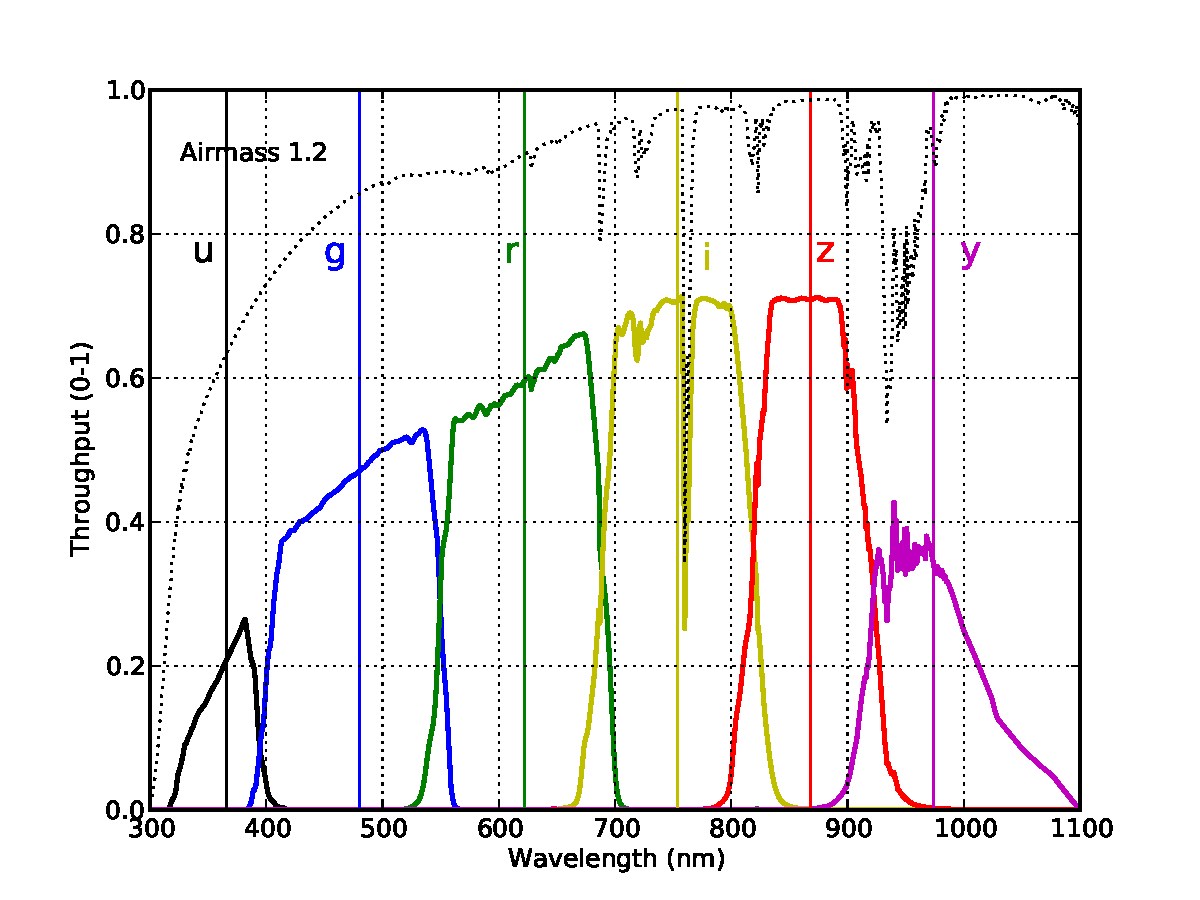
\includegraphics[width=5in]{filters}
\end{figure}


\section{Table of error budgets}

presumably the text motivates these, but this provides a place to
gather them, maybe add some more comments


\section{Potential improvements to photometric accuracy}

For scientists interested in higher precision photometry for objects
with known SEDs, it is possible to improve the procedure above, by
using the measured $S_b$ and their known SED to reconstruct the
expected counts. (even possibly redoing the flat field??)
\begin{equation}
F_v(\lambda) = F_o \, f_v(\lambda)
\end{equation}
where $f_v(\lambda_b)=1$ at some reference wavelength, $\lambda_b$,
chosen to be the effective wavelength of the standard bandpass
$\phi_b^{std}$.  

%\section{Comparison of standard calibration and SDSS ubercal (as
% approximation for this method)}


%\section{Thermal IR Camera}
%possibility to generate measurement of shape of cloud structure over
%field of view (could function as prior for self-calibration)

%if cloud structure found to vary on scales smaller than length between
%calibration stars (or minimum scale possible to correct with
%self-calib), then thermal IR camera would enable generation of
%these corrections

%may provide useful SDQA data (especially for alerts/nightly data
%stream)


\end{document}